\documentclass[11pt,spanish,a4paper]{article}

% Versión 1.er cuat 2021 Víctor Bettachini < vbettachini@unlam.edu.ar >

\usepackage[T1]{fontenc}
\usepackage[utf8]{inputenc}

\usepackage[spanish, es-tabla]{babel}
% \def\spanishoptions{argentina} % Was macht dass?
% \usepackage{babelbib}
% \selectbiblanguage{spanish}
% \addto\shorthandsspanish{\spanishdeactivate{~<>}}


\usepackage{graphicx}
\graphicspath{{./figuras/}{../LaTeX/}{../figurasLaTeX/}}
% \usepackage{float}

\usepackage[arrowdel]{physics}
\newcommand{\pvec}[1]{\vec{#1}\mkern2mu\vphantom{#1}}
% \usepackage{units}
\usepackage[separate-uncertainty= true, multi-part-units= single, range-units= single, range-phrase= {~a~}, locale= FR]{siunitx}
\usepackage{isotope} % $\isotope[A][Z]{X}\to\isotope[A-4][Z-2]{Y}+\isotope[4][2]{\alpha}

\usepackage{tasks}
\usepackage[inline]{enumitem}
% \usepackage{enumerate}

\usepackage{hyperref}

% \usepackage{amsmath}
% \usepackage{amstext}
% \usepackage{amssymb}

\usepackage{tikz}
\usepackage{tikz-3dplot}
\usepackage{tikz-dimline}
\usetikzlibrary{calc}
% \usetikzlibrary{math}
\usetikzlibrary{arrows.meta}
\usetikzlibrary{snakes}
\usetikzlibrary{decorations}
\usetikzlibrary{decorations.pathmorphing}
\usetikzlibrary{patterns}

\usepackage[hmargin=1cm,vmargin=3cm, top= 0.75cm,nohead]{geometry}

\usepackage{lastpage}
\usepackage{fancyhdr}
\pagestyle{fancyplain}
\fancyhf{}
\setlength\headheight{28.7pt} 
\fancyhead[LE, LO]{\textbf{Mecánica Analítica Computacional} }
% \fancyhead[LE, LO]{\textbf{Mecánica General} }
\fancyhead[RE, RO]{\href{https://ingenieria.unlam.edu.ar/}{$\vcenter{\hbox{
\includegraphics[height=1cm]{ambos.pdf}}}$}}
\fancyfoot{\href{https://creativecommons.org/licenses/by-nc-sa/4.0/deed.es_ES}{$\vcenter{\hbox{
\includegraphics[height=0.4cm]{by-nc-sa_80x15.pdf}}}$} \href{https://ingenieria.unlam.edu.ar/}{DIIT - UNLaM}}
\fancyfoot[C]{ {\tiny Actualizado al \today} }
\fancyfoot[RO, LE]{Pág. \thepage/\pageref{LastPage}}
\renewcommand{\headrulewidth}{0pt}
\renewcommand{\footrulewidth}{0pt}


\begin{document}
\begin{center}
  \textsc{\large Mecánica general}\\
  \textsc{\large Cinemática y dinámica Newtoniana de la partícula puntual}
\end{center}

%De poder resolver estos problemas en forma autónoma puede asumir que adquirió los conocimientos mínimos sobre los temas abordados.
%No dude en consultar a docentes y compañeros si no puede terminarlos.
% Los problemas marcados con * son opcionales.
\begin{enumerate}


\subsection*{Ecuaciones de la dinámica - 2"a ley de Netwon}
\item
\begin{minipage}[t][6.5cm]{0.6\textwidth}
\textbf{Marion e.g. 2.10} Particula cargada en \(\va{B}\) constante

La fuerza de Lorentz es la ejercida a una particular de carga eléctrica \(q\) por un campo eléctrico \(\vec{E}\) y magnético \(\vec{B}\):
\[
	\vec{F}= q \left( \vec{E}+ \vec{v} \cross \vec{B} \right).
\]
La figura muestra esquemáticamente una trayectoria y las condiciones \(\va{v}_0, \va{B}=\mathrm{cte}.\) que le dieron lugar.
Halle las ecuaciones de tal dinámica.
\end{minipage}
\begin{minipage}[c][0cm][t]{0.35\textwidth}
	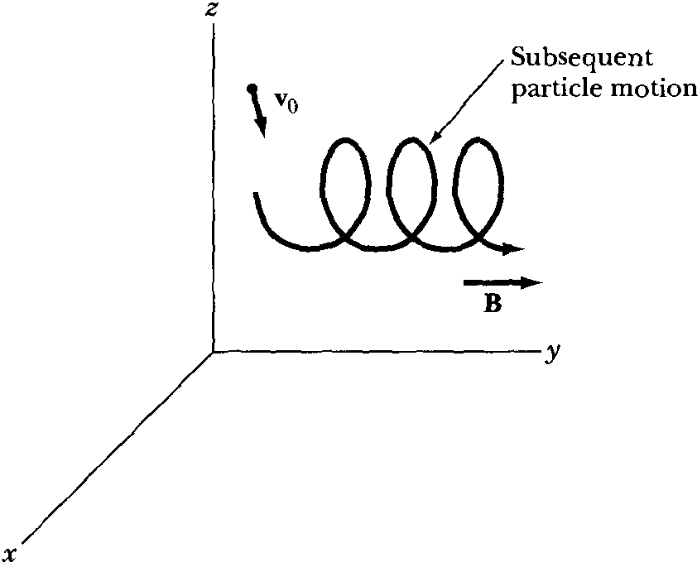
\includegraphics[width=\textwidth]{marionFig2_12.png}
\end{minipage}

\vspace{-2.5cm}



\subsection*{Condiciones de vínculo}
\vspace{-1cm}
\item
\begin{minipage}[t][4cm]{0.4\textwidth}
\textbf{Marion e.g. 2.9} Máquina de Atwood 

Esta máquina consiste de una polea sin fricción de la que suspenden dos masas al final de cada extremo de un hilo.
Encuentre la aceleración de las masas y la tensión de las cuerda:
  \begin{enumerate}
	\item cuando el centro de la polea está en reposo
	\item y cuando la polea desciende en un ascensor con aceleración constante \(a\).
  \end{enumerate}
\end{minipage}
\begin{minipage}[c][2cm][t]{0.55\textwidth}
	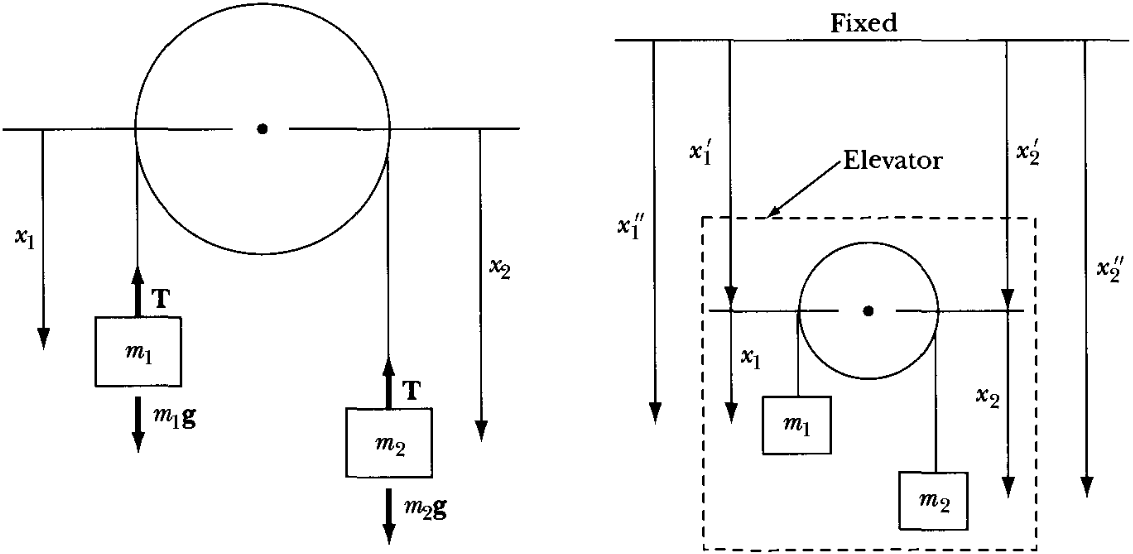
\includegraphics[width=\textwidth]{marionFig2_11.png}
\end{minipage}

%
%\item
%\begin{minipage}[t][3.5cm]{0.75\textwidth}
%Máquina de Atwood % \textbf{Vizcaino 1.1} 
%
%El sistema de la figura esta inicialmente en reposo, las poleas tienen masa despreciable y los hilos son inextensibles.
%  \begin{enumerate}
%   \item Halle la aceleración de cada cuerpo y las tensiones en los hilos en función de \(m_1\), \(m_2\), \(m_3\), y \(g\).
%   \item Resuelva a) para el caso \(m_1= \SI{4}{\kilo\gram}\), \(m_2= \SI{2}{\kilo\gram}\) y \(m_3= \SI{1}{\kilo\gram}\).
%  \end{enumerate}
%\end{minipage}
%\begin{minipage}[c][0em][t]{0.15\textwidth}
%        \includegraphics[width=\textwidth]{atwood-prob}
%\end{minipage}

\vspace{1cm}
\subsection*{Conservación: momento lineal}

% FCEyN 0.1
\item Dos masas \(m_1\) y \(m_2\) están unidas por una barra.
Se la coloca sobre una superficie horizontal sin rozamiento tal que la masa \(m_1\) la toque pero no la \(m_2\). 
Si se la deja en libertad, ¿donde golpea \(m_2\) a la superficie?


\subsection*{Conservación: momento angular}
\item \textbf{Marion e.g. 2.9}
Un ratón de masa \(m\) salta desde el borde externo de un ventilador de techo con momento de inercia \(I\) y radio \(R\).
¿Cuál es la razón de cambio de la velocidad angular?


%\subsection*{Momento angular}
%% FCEN 0.6
%% Problema horripilante, pues se resuelve como uno de fuerza central, hay que encontrar uno mas simple sobre conservación de momento angular.
%\item Dos partículas de masas \(m_a\) y \(m_b\) están sobre una mesa horizontal sin fricción.
%Se encuentran unidas por una cuerda tensa que pasa por un anillo pequeño fijo a la mesa, que tampoco presenta fricción a la cuerda. Inicialmente las partículas están quietas a distancias \(R_a\) y \(R_b\) del anillo y en \(t = 0\) se le da un impulso a la masa \(m_b\), perpendicular a la cuerda, de modo que esta adquiere una velocidad \(v_0\).
%\begin{enumerate}
%    \item ¿Qué magnitudes se conservan?
%    \item Dar la velocidad de las partículas en función de su distancia al anillo.
%    \item Hallar la tensión de la cuerda en función de la distancia de una masa al anillo.
%\end{enumerate}
%

\subsection*{Coordenadas polares}

% Vizcaino 1.12
\item Una masa m, considerada puntual, desliza sobre una semiesfera de radio R sin fricción.
	\begin{center}
  		\begin{tikzpicture}[scale= 1.3]
			\draw [ultra thick] (-3.5,0) -- (3.5,0);
			\fill [pattern = north east lines] (-3.5,0) rectangle (3.5,-0.2); % piso
			\draw [ultra thick] (-2,0) .. controls (-2,2*0.555) and (-2*0.555,2) .. (0,2)
			.. controls (2*0.555,2) and (2,2*0.555) .. (2,0); % semi esfera
			% \filldraw (0,2.2) circle (0.2); % masa superior
			\filldraw (2*0.5+.15,1.732+.15) circle (0.2) node [above, right=5] {\(m\)}; % masa a la derecha
			\draw (0,0) -- (0,2); % linea vertical
			\draw [->] (0,0) -- (1,1.732) node [anchor=center, below=10] {\(R\)}; % linea hacia la derecha
			\draw [->] (0,1) arc (90:60:1) node [above left] {\(\theta\)}; % arco c/ flecha comenzando en (0,1), de 90 a 60 grados, 1...
			% \node [circle,draw,label=60:$60^\circ$,label=below:$-90^\circ$] {\(m\)}; 
			% \node at (-2*0.5+.15,1.732+.15) [circle,draw,fill=black] {\(m\)}; 
			\draw [->] (-2.5,2) -> (-2.5,1) node [above=15, right=2] {\(\vec{g}\)}; % g vertical
	    \end{tikzpicture}
	\end{center}
  \begin{enumerate}
  \item Calcular el ángulo \(\theta\) para el cual se separa de semi-esfera si inicialmente la masa es apartada en un ángulo muy pequeño de \(\theta= 0\) y su velocidad inicial es nula.
  \item Si la masa \(m\) se engarza en el riel semicircular sin fricción de radio \(R\), hallar la velocidad con que llega al suelo.
¿Qué aceleración tangencial tiene \(m\) en ese momento?
  \end{enumerate}



% \section*{Sistema no inercial - sistema en rotación}
% % FCEyN 0.4
% \item Un disco homogéneo de masa \(M\) y radio \(R\) está girando con velocidad angular \(\omega \).
% % Una mosca de masa \(m\) que inicialmente se encuentra en el centro del disco camina radialmente hacia afuera con velocidad relativa constante.
% \begin{enumerate}
% \item Si el disco es obligado a girar con velocidad relativa constante por un motor, ¿qué torque debe hacer éste para compensar el movimiento de la mosca?
% ¿Cúal es la fuerza de Coriolis que siente la mosca?
% \item Si el disco gira libremente, ¿cúal será la velocidad angular del disco cuando la mosca está a una distancia \(d\) del centro?
% \end{enumerate}


%\item \setlength{\parskip}{0cm} % OLVIDÉ DE QUE TRATA ESTE PROBLEMA
%  \begin{enumerate}
%  \item Considere un resorte de constante elástica \(k\), sin masa y sin rozamiento, fijo de un extremo y obligado a moverse según una fuerza \(F_1\) de tal modo que \(x = x_0 \cos(\omega t)\)
%¿Cuánto debe valer \(F_1\)? (\(x\) se mide desde la posición de equilibrio).
%  \item Un cuerpo de masa \(m\) es movido por una fuerza \(F_2\) de tal modo que \(x = x_0 \cos(\omega t)\), ¿Cuánto vale \(F_2\)?
%  \item La masa \(m\) de b) se fija al extremo libre del resorte de a), y el sistema es obligado a moverse por una fuerza \(F_3\) de tal modo que la masa ejecuta un movimiento \(x = x_0 \cos(\omega t)\) ¿Cuánto vale \(F_3\)?
%  \item Si \(\omega = \omega_0 = \sqrt{\frac{k}{m}}\), ¿Cuánto vale \(F_3\)?
%  \item Estudie los límites \(\omega \gg \omega_0\) y \(\omega \ll \omega_0\), determine \(F_3\) y diga si el sistema se comporta como en a) o como en b).
%  \end{enumerate}

%
%\subsection*{Fuerza como gradiente de un potencial}
%% Vizcaino carpeta
%\item Una partícula esta sometida a una fuerza \(\vec{F}(x)= \left( -k x + \frac{a}{x^3}\right) \hat{x}\)
%\begin{enumerate}
%    \item Hallar el potencial \(U(x)\) y graficarlo.
%    \item Discutir los tipos de movimientos posibles.
%    \item Determinar las posiciones de equilibrio estable y encuentre la solución general de la dinámica de la partícula, \(\vec{r}(t)\).
%    \item Interpretar el movimiento en el límite \(E^2 \gg k a\). ¿Cuanto vale el periodo de las oscilaciones?
%    \item Ídem. anterior en el límite \(E^2 \rightarrow k a\) con \(E^2 > k a\).
%\end{enumerate}
%
\end{enumerate}
\end{document}
